
\documentclass[journal]{IEEEtran}

\usepackage{graphicx}
\usepackage[utf8]{inputenc}
\usepackage{algorithm}
\usepackage{algorithmic}
\usepackage{amsmath}
\usepackage{amssymb}

%\usepackage[noend]{algpseudocode}

%\usepackage[noend]{algpseudocode}

%\restylefloat{algorithm}



\begin{document}
 
\title{\textbf{handling learnability imbalance in multiclass-classification}}



\author{Theodor Peifer
        \linebreak
        email: thp7219@thi.de
        \linebreak
        Technische Hochschule Ingolstadt
}



\maketitle


\begin{abstract}
Neural Networks have proven themselves to be powerful classification
tools by solving problems in a range of domains with high accuracy.
Yet this accuracy is never evenly distributed across all classes, which means that the true-positive rates of each class separately are different.
This can happen even in balanced datasets since some classes are more difficult to learn by the model than others (this phenomenon is further referred to as \emph{learnability-imbalance}).
A common way to address this problem is to give a weight to the error function for each class to penalize losses of certain classes higher or lower.
This research will address the determination of such weights to counteract the learnability-imbalance in balanced datasets using previously calculated evaluation scores.
Therefore the goal is to find methods to lower the variance of the true positive rates of each class.
\end{abstract}


\section{Introduction}
A frequent problem in classification appears when working with datasets that have an unequal amount of samples per class and are therefore called a \emph{class imbalanced} datasets. %, where \emph{classes} describe the categories which the model has to classify.
Since there will be some classes, that have less elements for the model to learn from, their features will be harder to extract what finally will result in a lower true positive rate, i.e. a per-class accuracy [1].
Thus, the consequence of having different class sizes can be described as having a \emph{learnability imbalance} in the dataset since some classes are more difficult to learn that others.
%Classes with less element are harder to learn, which won't only result in big differences in the true positive rates [1] of the individual classes but also in a lower, overall accuracy.
%In order to prevent this, it is common to weight the error function [1] according to the size of each class, i.e. the number of samples it contains.
%Therefore, for every class there is a weight, which is greater the fewer elements it contains and that gets multiplied with the loss produced by its samples. % "Therefore" wrong
%Since the aim of a neural network is to minimize the overall loss and samples from a smaller class will produce a higher error, they will have a higher impact on the learning process in order to compensate for the different class sizes.

% , samples from that produce a high loss will have a higher impact on the learning process.
% This can prevent the model from learning the patterns of a class with less element worse than others.
% With the evaluation a set of true positive rates can be calculated for each class which reveals what classes are more difficult to learn by the model and should have received a higher weight. 

But such learnability differences can appear also in balanced datasets for a variety of reasons, e.g. when the quality of the data of a class is lower than the rest of the data % or when the classes come not from the distributions. 
A second reason, that this research will be focused on, is that when some classes are similiar, % "similiar objects"?
the model can confuse their samples with each other more easily what will often result in a lower accuracy of those classes.
%This issue is an inevitable product of every normal classification.

%This issue is a light version of the imbalanced dataset problem and the inevitable product of every normal classification. 
Even though this issue is an inevitable product of every normal classification, in most cases the learnability difference of the classes is either low or not from great interest.
But there can be more extreme cases where the model needs to produce fair and unbiased results using a dataset that has an obvious learnability imbalance. 
An example is \emph{name-ethnicity classification}, where a model predicts the ethnicity of a name only by its letters [5]. 
Nationalities that use the same language and therefore have similiar names (e.g. \emph{british} and \emph{american}) result in a lower accuracy (see figure 1).
Thus, when a model that is trained on such a dataset is used, e.g. for social science experiments, it can produce unfair and biased results. 

\begin{figure}[h!]
        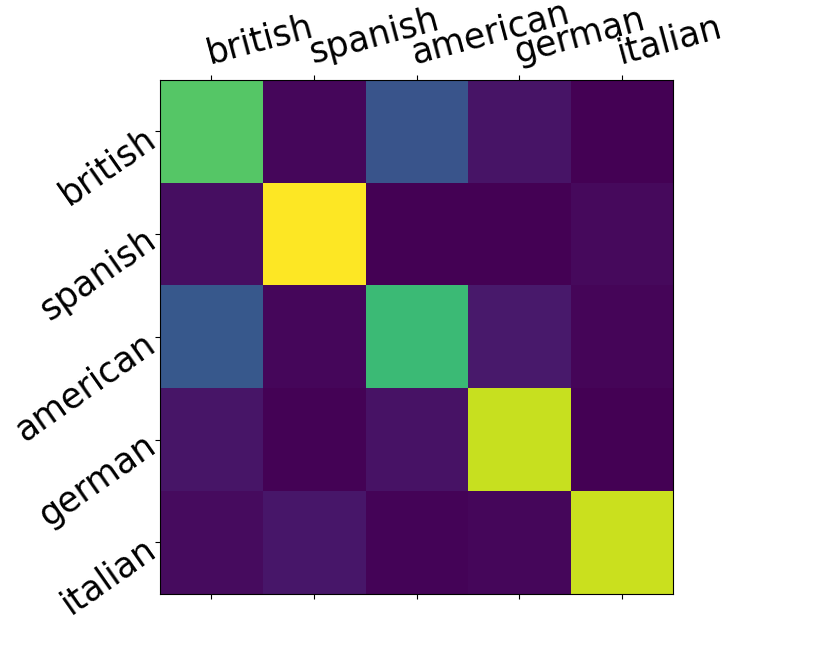
\includegraphics[width=\linewidth]{images/Figure_1.png}
        \caption{confusion matrix representing the true positive distribution of the name-nationality dataset produced by a recurrent neural network}
        \label{fig:tp_scores}
\end{figure}

Another dataset that is a good showcase for the learnability imbalance is the CIFAR-10 [2] dataset (32$\times$32 RGB images of ten different classes) because it also contains similiar classes such as \emph{dog} and \emph{cat}.
%Another dataset that is a good showcase for the learnability imbalance is the CIFAR-10 [2] dataset because in the 10 different classes which consist of 32x32 pixel images, there are also similiar ones such as \emph{dog} and \emph{cat}.
When looking at the true positive rates produced by a convolutional neural network [3], trained on that dataset, it can be seen that there are some classes that got misclassified more often (in this case bird, cat, deer and dog) which hints to a more difficult learnability. 
The CIFAR-10 and the name-nationality dataset will be used for experiments in order to find methods for minimizing such variances in the evaluation scores.

%\begin{figure}[h!]
%        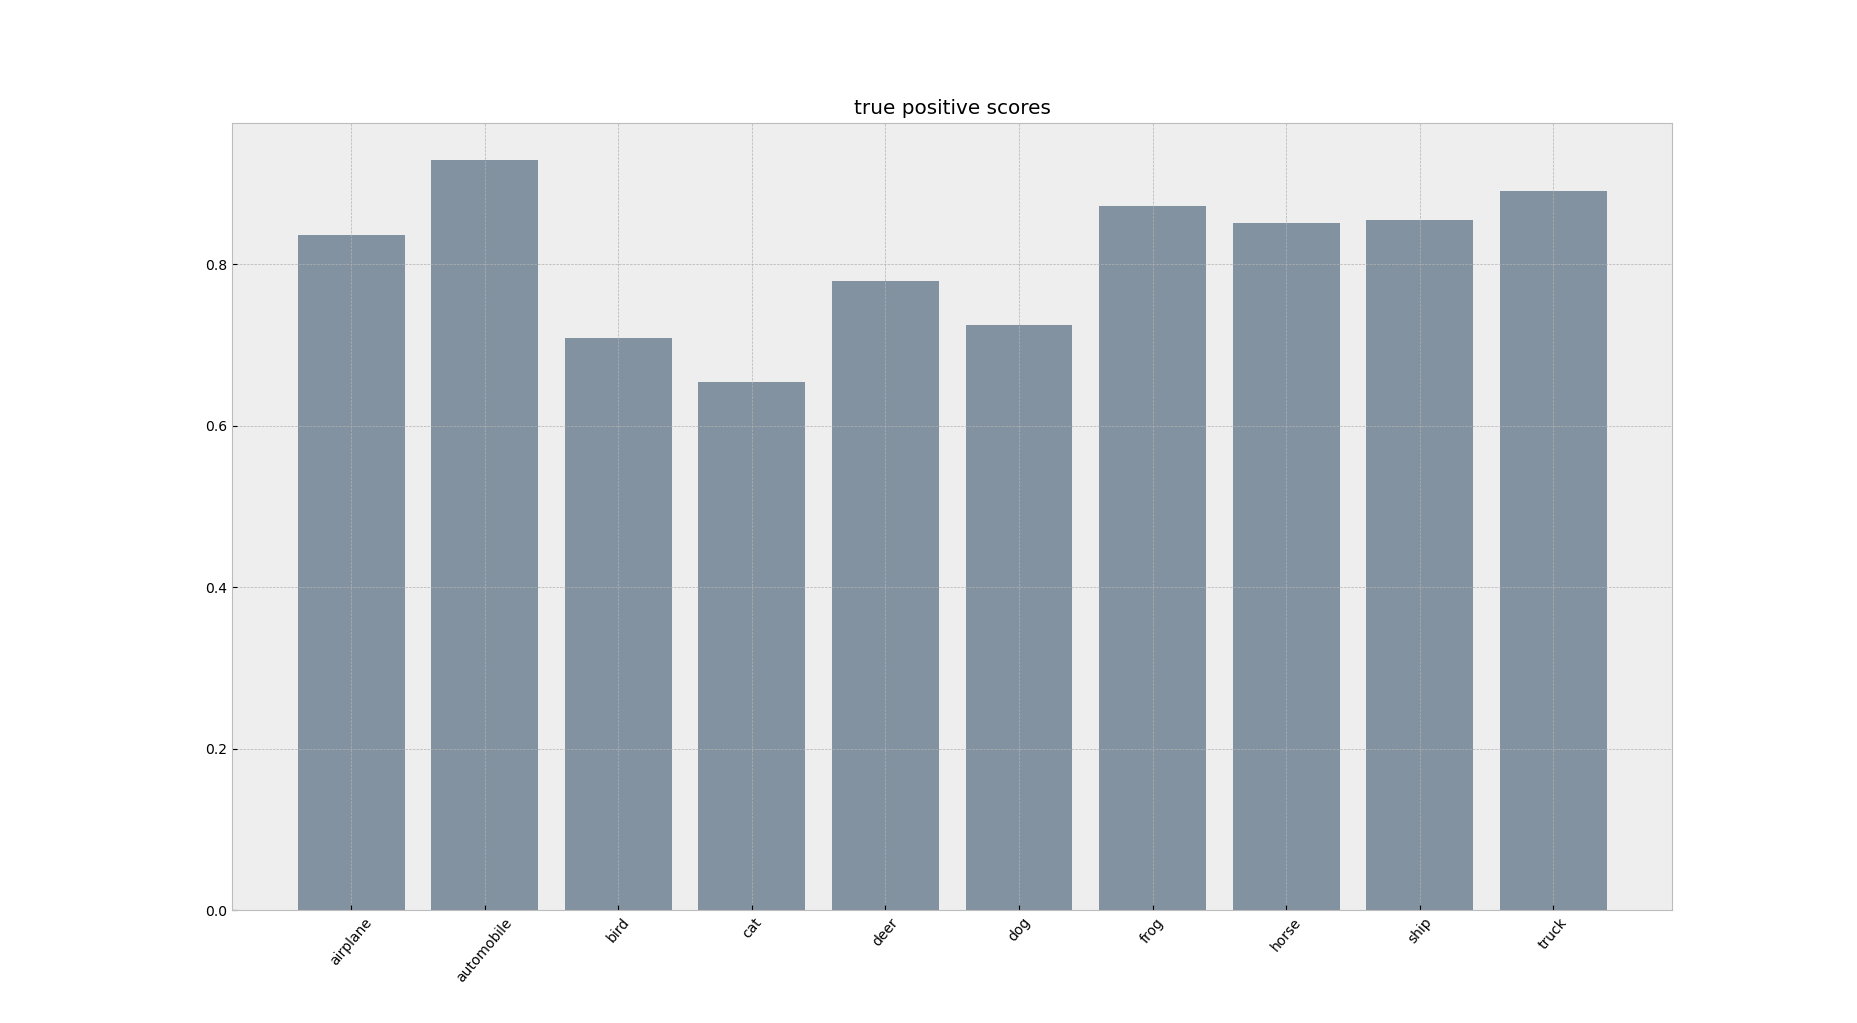
\includegraphics[width=\linewidth]{images/cifar10_tp_scores.png}
%        \caption{true positive scores of a model trained on the CIFAR-10 dataset}
%        \label{fig:tp2_scores}
%\end{figure}

%---> When working with such datasets the learnability differences of the individual classes are mostly only identifiable after the model has been trained and evaluated normally.
%---> A confusion matrix or the calculation of the true positive rates then reveal what classes where learned the best and which should have received a higher weight. 

To figure out such methods one should first go back to the class imbalance problem because there are already solutions existing.
One of which is to weight the error function [1] according to the size of each class, i.e. the number of samples it contains.
Therefore, for every class there is a weight, which is greater the fewer elements it contains and that gets multiplied with the loss produced by its samples. % "Therefore" wrong
%Since the aim of a neural network is to minimize the overall loss and samples from a smaller class will produce a higher error, they will have a higher impact on the learning process in order to compensate for the different class sizes.
That will cause, that samples from a smaller class will produce a higher error and, since the aim of a neural network is to minimize the loss [4], will have a higher impact on the learning process.

Other methods will be discussed when reviewing exisiting literature on this topic. 
%Another way to try to compensate for the different class sizes is to use more augmentation [5] on the samples of smaller classes. 
%Augmentation describes the random transformation of the samples, in order to synthetically generate more input data for the model. For example, in image classification it is common to randomly flip, mirror or to add white noise to the images [6].
But since all of those approaches rely on the different proportions of the classes in the dataset it raises the question how to apply them on datasets that, even though they don't suffer from class imbalance, still show a big learnability imbalance.
When working with such datasets the learnability differences of the individual classes are mostly only identifiable after the model has been trained normally und unweighted. % and without any regard for the potential imbalance of the dataset. 
The calculation of the true positive rates and visualization (e.g. confusion matrix) can then reveal what classes were learned the best and which should have received a higher weight.
These evaluation scores can then be used to determine which loss weights or how much data augmentation should be used for each class (an example is shown in \emph{algorithm 1}).

In summary, this research will focus on creating and testing methods which use the true positive rate of each class in order to find out how much a class should be weighted or augmentated in order to counteract the learnability imbalance of the dataset.

%The aim is to increase the accuracy of classes which originally had a low one and decrease the accuracy of those which had a higher one, without decreasing the true positive rate of the whole test set 
%(this can described as the per-class accuracies "meeting up in the middle" where the original overall accuracy lied).
The aim is to bring all per-class accuracies to the same value by increasing the true positive rate of classes that are harder to learn 
and decrease the rate of classes that more easily to learn.
Further, it will address potential limitations and risks such as the reduction of the overall accuracy that could potentially happen from this process.
%This research will test which methods can be applied on the model with respect to the per-class rates.
%Alogrithm 1 proposes a method to use true positive rates in order to create a set of loss weights which should be used to re-train the model with a higher focus on classes which a more difficult to learn.
%The evaluation of that model will then produce a set that contains the score of each class, which will then

\begin{algorithm}[H]
        \caption{creating loss weights for a balanced dataset}

        \textit{\textbf{C} $\hat{=}$ amount of classes}
        %\\ \textit{\textbf{train(weights)} describes the initialization and the whole training process of a classification model using the loss-weights $weights$. \\$weights_i$ will be multiplied to every loss generated by a sample of class $i$.}
        \\ \textit{\textbf{train(weights)} describes the initialization and training process of a classification model in which $weights_i$ will be multiplied to every loss generated by a sample of class $i$.}
        \\ \textit{\textbf{evaluate()} creates the set $s$ with $\left|s\right|$ = $C$ and $s_i \in [0;1]$ which contains the true positive scores of all classes of the test dataset.}
        \\ \textit{\textbf{W(s)} is a function that creates a set of loss-weights $w$ with $\left|w\right|$ = $C$ and $w_i \in \mathbb{R}^{+}$ using a set of true positive scores $s$: $W: [0;1] \rightarrow \mathbb{R}^{+}$ ; $\{s_i,...,s_C\} \rightarrow \{w_i,...,w_C\}$ }
        \\ \textit{\textbf{process:}}
        \begin{algorithmic}[1]
         \STATE $train(weights\texttt{=}\{w_1\texttt{=}1, w_2\texttt{=}1, ..., w_C\texttt{=}1\}$)
         \STATE $s = evaluate()$
         \STATE $w = W(s)$
         \STATE $train(weights\texttt{=}w)$
         \STATE $s' = evaluate()$
         \STATE $compare(s, s')$

        \end{algorithmic}
\end{algorithm}


\section{literature review}
%Since the term \emph{learnability imbalance} is proposed for this research, it's pointing out the fact that this, for most cases ignorable, problem is barely addressed directly.
%But as mentioned before, the possible solutions are the same as for the class imbalanced dataset problem which itself causes learnability imbalance.
%Therefore to find methods
As mentioned before, the learnability imbalance has to be handled the same way as the class imbalanced dataset problem, but by using the true positive rates instead of the class proportions of the dataset.
%Therefore, this research overlaps very much with the research about class imbalance and will make use its proposed solutions.
Therefore, the proposed solutions to class imbalance are fundamental to this research and will be reviewed in the following (the methods in summary: loss weighting, augmentation and over-/ undersampling).

Since it was used as a main example in the introducion, the first method to examine is loss weighting [N]. 
This approach has proven itself to be a good way for archieving a lower variance in the per-class accuracies of unbalanced datasets and will be adapted to this research. 
In general, the weights are chosen to be inversely proportional to the amount of samples in the classes [Na].
The following formula 1 shows a proposed weight determination function of the paper [N]:

\[ w_c = \frac{1-\beta^{N_c}}{1-\beta} \]

This methods gets described as the \emph{effective number of samples} weight, where $N_c$ is the amount of samples of class $c$ and $\beta$ is a tuneable hyper-parameter with $\beta \in [0;1[$ .

Formula 2 shows how to use such weights along with the cross entropy loss function [N] for one sample:
%\[ \text{L}(x, c) = w_{c} \cdot \left(-\log\left(\text{P}(y_c|x, \theta)\right) \right) \]
\[ \text{CE}(x, c) = w_{c} \cdot \left(-\log\left(\hat{y}_c)\right) \right) \]

%\[ \text{L}(x, c) = w_{c} \cdot \left(-\log(\hat{y_c}) \right) \]
%\[ loss(x, class) = w_{class} * \left(-log\left(N(x, \theta)_{class}\right) \right) \]

%$\hat{y} := \{p_1, ..., p_C | C \hat{=} amount of classes\}$ is a probablity distribution and the output of a model $\text{F}(x, \theta)$ with learnable parameter $\theta$ and $C$ is the amount of classes.
%Then $\hat{y_c}$ represents the confidence of the model that an input sample $x$ is corresponds to the correct class $c$.

$\hat{y}$ is the output of a model $\text{F}(x, \theta)$ with learnable parameter $\theta$ and can be described as a probability distribution for which $\hat{y_i}$ is the confidence of the model, that the input sample $x$ corresponds to the $i$-th class.
Therefore $\hat{y_c}$ represents the probability that the model correctly classified $x$ as the wanted class $c$. 
As shown, the weight $w_c$ that corresponds to the correct class gets multiplied with the normal error value (in the case of cross entropy: the negative $\log$ of the probablity).

%$\text{P}(y_c|x, \theta)$ is the confidence of a model $\text{F}(x, \theta)$ with learnable parameter $\theta$ that an input sample $x$ corresponds to the correct class $y_c$.
%$\text{F}(x, \theta)$ outputs a probablity distribution which represents the confidence of every class and has the property $\sum_{i=0}^{C-1}P(y_i|x,\theta) = 1$ by using the softmax activation function [N]. The loss is then calculated by taking the negative $\log$ of only the probablity of the wanted class.

Another loss weighting method is the so called \emph{focal loss}, which is especially interesting for this research because it uses the true positive rates instead of the sizes of the classes to generate the weights.
But since it is also mainly tested and practiced on class imbalanced datasets, this research will investigate its effectiveness on class balanced datasets that have a learnability imbalance.
The weight for the focal loss is defined as the following ($\gamma$ is a positive hyperparameter for scaling):
\[ w_c = (1 - \hat{y}_c)^\gamma \]

When multiplying this weight with the loss, it will be bigger, the smaller the confidence of the correct class was. 
The adavantage of the focal loss over the proposed weight generation of this research is that it does not require a pre-training in order to figure out which classes a harder to learn, since it does this during the training process.
But a hypothesis is, that this weighting could have less impact on learnability imbalanced datasets because it figures out the imbalance while training.
In contrast to this, when training unweighted first, calculating the weights afterwards and training again with those weights, the loss function can start penalizing the classes differently from the beginning.

%\[ \text{L}(x, c) = w_{c} \left(-y_{c} \cdot \log\left(N(x, \theta)\right) \right) \]


%The formula 1 above represents the weighted cross entropy loss where $x$ is an input sample and $y_{class}$ the integer representation of the corresponding class with $y := \{0, ..., C-1\}$.
%$N(x, \theta)$ is the output of the model with the learnable parameters $\theta$ and can be described by a probablity distribution $P(y|x,\theta)$. $P(y_{class}|x,\theta)$ represents the confidence of the model that sample $x$ corresponds to class $class$ with the property $\sum_{i=0}^{C-1}P(y_i|x,\theta) = 1$.
%$\left|N(x, \theta)\right| = C$ is the probablity distribution calculated using the learnable parameters $\theta$.
%The output $P(x|\theta) = N(x, \theta)$ is a probablity distribution with $\left|N(x, \theta)\right| = C$  $P(x = i|\theta)$ is the probablity that the input $x$ corresponds to class $i$.

\section{approach}
TODO second section here

\section{third section}
TODO third section here

\begin{thebibliography}{1}

\bibitem{}
Name Name, Name Name, Name Name (2006). Title, 24(1), 29-33.

\end{thebibliography}

\end{document}

% biased class distribution: https://link.springer.com/chapter/10.1007/3-540-44795-4_45#:~:text=Labeled%20data%20for%20classification%20could,optimal%20classification%20on%20new%20data.
% class imbalance over sampling: https://machinelearningmastery.com/random-oversampling-and-undersampling-for-imbalanced-classification/
% CEL: https://arxiv.org/ftp/arxiv/papers/2001/2001.00570.pdf
% a: https://arxiv.org/pdf/1901.05555.pdf (p 4)
% focal loss: https://arxiv.org/pdf/1708.02002.pdf